\let\negmedspace\undefined
\let\negthickspace\undefined
\documentclass[journal]{IEEEtran}
\usepackage[a5paper, margin=10mm, onecolumn]{geometry}
%\usepackage{lmodern} % Ensure lmodern is loaded for pdflatex
\usepackage{tfrupee} % Include tfrupee package

\setlength{\headheight}{1cm} % Set the height of the header box
\setlength{\headsep}{0mm}     % Set the distance between the header box and the top of the text

\usepackage{gvv-book}
\usepackage{gvv}
\usepackage{cite}
\usepackage{amsmath,amssymb,amsfonts,amsthm}
\usepackage{algorithmic}
\usepackage{graphicx}
\usepackage{textcomp}
\usepackage{xcolor}
\usepackage{txfonts}
\usepackage{listings}
\usepackage{enumitem}
\usepackage{mathtools}
\usepackage{gensymb}
\usepackage{comment}
\usepackage[breaklinks=true]{hyperref}
\usepackage{tkz-euclide} 
\usepackage{listings}
% \usepackage{gvv}                                        
\def\inputGnumericTable{}                                 
\usepackage[latin1]{inputenc}                                
\usepackage{color}                                            
\usepackage{array}                                            
\usepackage{longtable}                                       
\usepackage{calc}                                             
\usepackage{multirow}                                         
\usepackage{hhline}                                           
\usepackage{ifthen}                                           
\usepackage{lscape}

\renewcommand{\thefigure}{\theenumi}
\renewcommand{\thetable}{\theenumi}
\setlength{\intextsep}{10pt} % Space between text and floats


\numberwithin{equation}{enumi}
\numberwithin{figure}{enumi}
\renewcommand{\thetable}{\theenumi}

% Marks the beginning of the document
\begin{document}
\bibliographystyle{IEEEtran}

\title{9.4.20}
\author{EE24BTECH11049 - Patnam Shariq Faraz Muhammed}

% \maketitle
% \newpage
% \bigskip
{\let\newpage\relax\maketitle}

\textbf{Question}:\\

In a bank, the principal continuously increases at a rate of $r\%$ per year. Find the value of $r$ if Rs 100 doubles in 10 years \brak{\log_e2 = 0.6931}.\\

\textbf{Solution: }\\

\begin{table}[ht!]
    \centering
    \begin{tabular}{|c|c|}
    \hline
    \textbf{Variable} & \textbf{Description}\\
    \hline
    $P_0$ & initial principal amount\\
    \hline
    $r$ & rate of increase per year\\
    \hline
    $t$ & time in years\\
    \hline 
    $C \& C_1$ & arbitrary constants\\
    \hline
    $P$ & principal at any time $t$\\
    \hline
\end{tabular}

    \caption{Variables used}
    \label{tab:my_label}
\end{table}

$P$ is the principal at any time, according to the given question, the rate of change of principal can be written as follows.

\begin{align}
    \frac{dP}{dt} &= \brak{\frac{r}{100}} \times P \label{1}
\end{align}

Separation of the variables in the equation \eqref{1}

\begin{align}
     \frac{dP}{p} &= \brak{\frac{r}{100}} \times dt \label{2}
\end{align}

Integration on both sides \eqref{2}

\begin{align}
    \int{\frac{dP}{p}} &= \int{\brak{\frac{r}{100}} dt}\\
    \log_e{P} &= \frac{rt}{100} + C\\
    P &= e^{\frac{rt}{100} + C}\\
    P &= e^{\frac{rt}{100}}e^C\\
    P &= C_1e^{\frac{rt}{100}} \label{3}
\end{align}

At time $t = 0$, it is given that the principal is $100$, that is, $P_0 = 100$. \\ 
Substitute in equation \eqref{3}

\begin{align}
    100 = C_1
\end{align}

Principal can be written as

\begin{align}
    P &= 100 \times e^{\frac{rt}{100}} \label{4}
\end{align}

At $t = 10$, the principal doubles, that is, $P = 200$, using equation \eqref{4}

\begin{align}
    200 &= 100 \times e^{\frac{r}{10}}\\
    2 &= e^{\frac{r}{10}}\\
    \log_e{2} &= \frac{r}{10}\\
    r &= 10 \times \log_e{2}\\
    r &= 6.931
\end{align}

The differential equation 
\begin{align}
    \frac{dP}{dt} &= 0.06931 \times P \label{diffeq}
\end{align}

\textbf{Verification of the solution computationally:}\\
\textbf{Euler's Method:}

From the definition of $\frac{dy}{dx}$,
\begin{align}
    \frac{dy}{dx} &\approx \frac{y\brak{x + h} - y\brak{x}}{h}\\
    \frac{dy}{dx} &= \frac{y_{n+1} - y_n}{h}
\end{align}

As per the question

\begin{align}
    \frac{dP}{dt} &= \frac{P_{n+1} - P_n}{h}
\end{align}

substitute \eqref{diffeq}

\begin{align}
    \frac{P_{n+1} - P_n}{h} &= 0.06931\times P_n
\end{align}

We represent the the differential equation in the following difference equations:

\begin{align}
    t_{n+1} &= t_{n}+h \\
    P_{n+1} - P_n &= 0.06931\times P_n \times h\\
    P_{n+1} &= P_{n}+h \times 0.06931 \times P_n
\end{align}
Where h is step and is small.

\textbf{Laplace transforms:}
\begin{itemize}
    \item If $f\brak{t}$ is a function, the Laplace transform of that function is
\begin{align}
    \mathcal{L}\brak{f\brak{t}} = \int_0^{\infty}{e^{-st}f\brak{t}}dt \label{lap}
\end{align}
    \item It is linear transformation, since integral is a linear operator 
    \item \textbf{Laplace tranforms of some functions:}
    \begin{align}
        f\brak{t} &= 0 \implies F(s) = 0 \\
	f\brak{t} &= 1 \implies F(s) = \frac{1}{s} \text{ for } Re(s) > 0\\
	f\brak{t} &= t^n \implies F(s) = \frac{\Gamma\brak{a+1}}{s^{n+1}} \text{ for } Re(s) > 0 \\
	f\brak{t} &= e^{at} \implies F(s) = \frac{1}{s-a} \text{ for } Re(s) > a \\
	f\brak{t} &= \sin{at} \implies F(s) = \frac{a}{s^2 + a^2} \text{ for } Re(s) > 0 \\
	f\brak{t} &= \cos{at} \implies F(s) = \frac{s}{s^2 + a^2} \text{ for } Re(s) > 0\\
        f\brak{t} &= \sinh{at} \implies F(s) = \frac{a}{s^2 - a^2} \text{ for } Re(s) > 0 \\
	f\brak{t} &= \cosh{at} \implies F(s) = \frac{s}{s^2 - a^2} \text{ for } Re(s) > 0\\
        f\brak{t} &= e^{\omega t}\sin{at} \implies F(s) = \frac{a}{(s-\omega)^2 + a^2} \text{ for } Re(s) > \omega  \\
	f\brak{t} &= e^{\omega t}\cos{at} \implies F(s) = \frac{s - \omega}{(s-\omega)^2 + a^2} \text{ for } Re(s) > \omega 
    \end{align}
    \item \textbf{Laplace transforms of derivatives:}
    \begin{align}
			\mathcal{L} \brak{f^{\prime}} &= s F(s) - f(0) \label{dif1} \\
			\mathcal{L} \brak{f^{\prime \prime}} &= s^2 F(s) - s f(0) - f^{\prime}(0) \label{dif2}
    \end{align}

    \item \textbf{Laplace transform of unit step function $u(t)$ :} \\
		\begin{align}
			u(t) &= 
			\begin{cases} 
			1 & t \geq 0 \\
			0 & t < 0
			\end{cases} \label{ut}
		\end{align}
			\text{From \eqref{lap}}
		\begin{align}
			\mathcal{L} \brak{u(t)} &= \int_{0}^{\infty} u(t) e^{-st} dt 
		\end{align}
		For all non-negative values, $u(t) = 1$. Hence, the integral becomes,
		\begin{align}
			F(s) &= \int_{0}^{\infty} (1)e^{-st} dt \\
			F(s) &= \left[ \frac{e^{-st}}{-s} \right]_{0}^{\infty} = \frac{1}{s} ,  \text{ for } Re(s) > 0 \label{eq:first}
		\end{align}
	\item \textbf{Laplace transform of $e^{at} u(t)$ :} \\
		From \eqref{lap}
		\begin{align}
			\mathcal{L} \brak{e^{at} u(t)} &= \int_{0}^{\infty} e^{at} u(t) e^{-st} dt \\
			F(s) &= \int_{0}^{\infty} e^{(a-s)t} dt \\
			F(s) &= \left[\frac{e^{(a-s)t}}{a-s} \right]_{0}^{\infty} = \frac{1}{s-a} , \text{ for } Re(s) > a \label{req}
		\end{align}
    \item \textbf{Solution for the differential equation:}\\
    Let $f\brak{t} = P\brak{t}$\\
    Apply Laplace transform to the equation \eqref{1}
    \begin{align}
        \mathcal{L}\brak{f^{\prime}} &= \mathcal{L}\brak{0.06931\times f}\\
    \end{align}
    From equations \eqref{dif2} and \eqref{dif1}
    \begin{align}
        sF\brak{s} - f\brak{0} &= 0.06931F\brak{s}\\
        \brak{s - 0.06931}F\brak{s} &= f\brak{0}\\
        F\brak{s} &= \frac{f\brak{0}}{s - 0.06931}
    \end{align}
    Substitute the initial conditions $f\brak{0} = 100$
    \begin{align}
        F\brak{s} &= \frac{100}{s - 0.06931}\\
        \mathcal{L}\brak{f\brak{t}} &= \frac{100}{s - 0.06931}\\
        f\brak{t} &= \mathcal{L}^{-1}\brak{\frac{100}{s - 0.06931}}\\
    \end{align}
    from equation \eqref{req}
    \begin{align}
        f\brak{t} &= 100\times u\brak{t}e^{0.06931t}\\
        P\brak{t} &= 100\times u\brak{t}e^{0.06931t}
    \end{align}
\end{itemize}

\textbf{Z-transform:}
\begin{itemize}
    \item If $f\brak{t}$ is a function, the Z-transform of that function is
    \begin{align}
        X\sbrak{z} = \mathcal{Z}\brak{x\sbrak{t}} = \sum_{t = -\infty}^{\infty} {x\sbrak{t}}z^{-t} \label{z}
    \end{align}
    \textbf{Z-transform of some functions}
    \item \textbf{$u(t)$} : \\
		From \eqref{z}
		\begin{align}
			Y(z) &= \sum_{t \to -\infty}^{\infty} u\sbrak{t} z^{-t} 
		\end{align}
		From \eqref{ut}, we simplify it as
		\begin{align}
		        Y(z) &= \sum_{t=0}^{\infty} (1)z^{-t} \\
			Y(z) &= \frac{1}{1 - z^{-1}}, \label{eq:zut} \text{ for } \abs{z} > 1 
		\end{align}
	   \item \textbf{$a^t u(t)$} : \\
		From \eqref{z} 
		\begin{align}
			X\sbrak{z} &= \sum_{t \to -\infty}^{\infty} a^t u\sbrak{t} z^{-t} 
		\end{align}
		From \eqref{ut}, we simplify it as
		\begin{align}
			X\sbrak{z} &= \sum_{t=0}^{\infty} a^t z^{-t} \\
			X\sbrak{z} &= \sum_{t=0}^{\infty} \brak{az^{-1}}^{t} 
            \end{align}
            \begin{align}
			X\sbrak{z} &= \frac{1}{1 - az^{-1}}, \text{ for } \abs{z} > \abs{a} \label{eq:atut}
		\end{align}
	\item \textbf{Some other useful results} : \\
		\begin{align}
			\mathcal{Z}\sbrak{u_{n-1}} &= z^{-1} \mathcal{Z}\sbrak{u_{n}} \\
			\mathcal{Z}\sbrak{u_{n+1}} &= z \brak{\mathcal{Z}\sbrak{u_{n}} - u_{0}}
		\end{align}
        \item \textbf{Solution:}
        from \eqref{equa}
        \begin{align}
            P_{n+1} &= P_{n}+h \times 0.06931 \times P_n\\
            P_{n+1} &= P_{n}\brak{1 + 0.06931h}
        \end{align}
        Apply z-transform
        \begin{align}
            \mathcal{Z}\sbrak{P_{n+1}} &= \mathcal{Z}\sbrak{P_{n}\brak{1 + 0.06931h}}\\
            \mathcal{Z}\sbrak{P_{n+1}} &= \brak{1+0.06931h}\mathcal{Z}\sbrak{P_{n}}
        \end{align}
        Let,
        \begin{align}
            \mathcal{Z}\sbrak{P_n} &=P\sbrak{z}
        \end{align}
    Then,
        \begin{align}
            \mathcal{Z}\sbrak{P_{n+1}} &=zP\sbrak{z}-zP_0
        \end{align}
    Now,
        \begin{align}
            zP\sbrak{z}-zP_0 &= P\sbrak{z}(1+0.06931h) \\
            P\sbrak{z} \sbrak{z-\brak{1+0.06931h}} &= zP_0 \\
            P\sbrak{z} &= P_0 \sbrak{\frac{z}{z-\brak{1+0.06931h}}}
        \end{align}
    By inversing, we get 
        \begin{align}
            P_n &= P_0 \times \brak{1+0.06931h}^n
        \end{align}
    We know that,
        \begin{align}
            1+0.06931h \approx e^{0.06931h}
        \end{align}
    then,
        \begin{align}
            P_n &= P_0 \brak{e^{0.06931h}}^n \\
            P_n &= P_o e^{0.06931nh}
        \end{align}
        As h is the small division of time and n are the total no.of divisions, nh turns to be t at that point,Then
        \begin{align}
            P\brak{t}=P_0e^{0.06931t}
        \end{align}
\end{itemize}

We iterate this by taking the initial conditions from $t = 0$ to $t = 10$\\
By plotting all the points \brak{t,P} we get the graph of function P varying with t.\\
The comparison between theoretical and simulation curves is shown in the figure, we can clearly see that both the curves are coincides which verifies our solution.\\
For the following approximate graph, I chose $h = 0.1$

\begin{figure}[H]
   \centering
   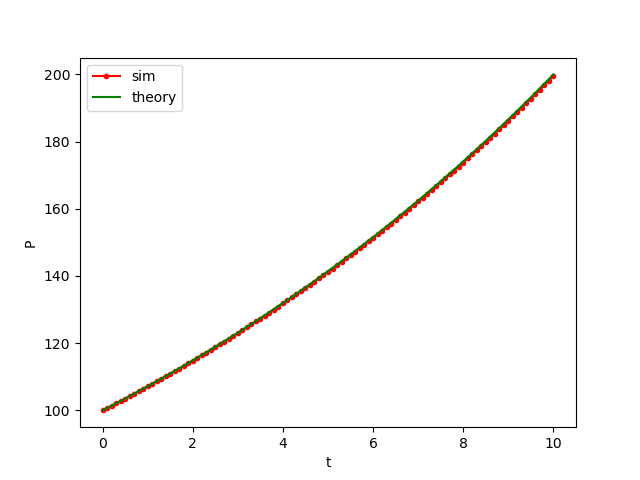
\includegraphics[width=0.7\columnwidth]{figs/fig.png}
    \caption{Approximate solution of the DE}
\end{figure}
\end{document}
